\begin{figure}
    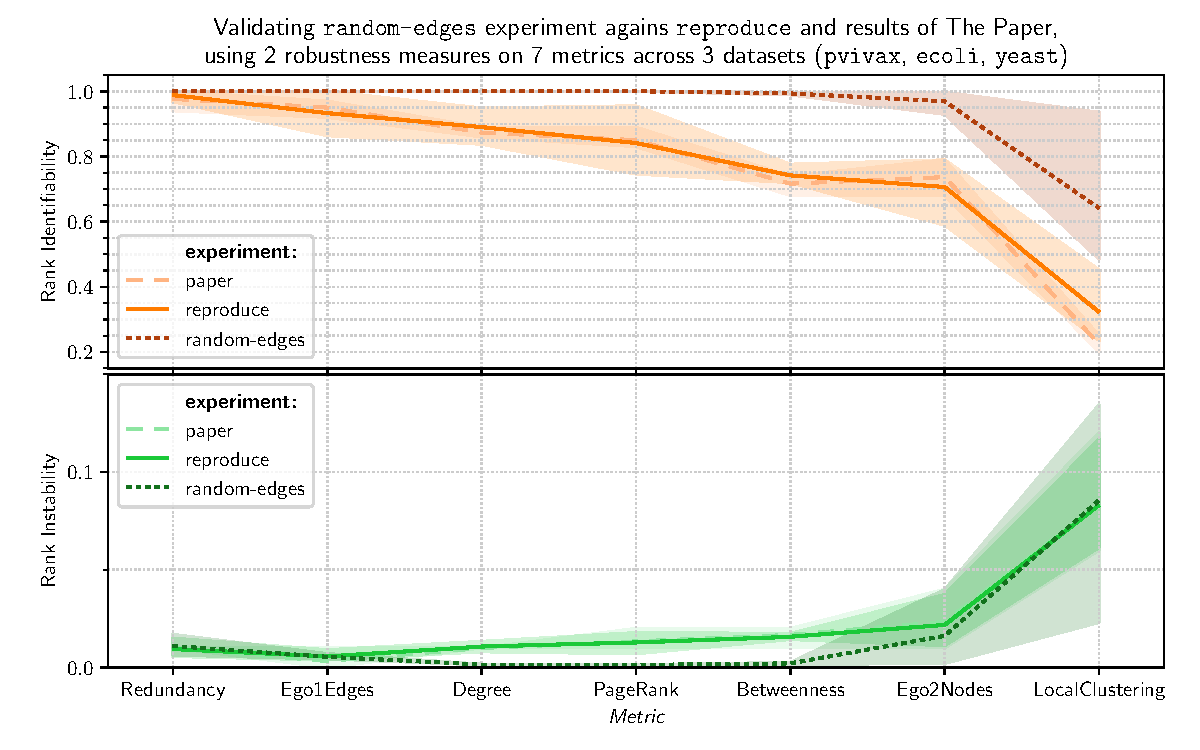
\includegraphics[width=\linewidth]{plot_random_edges.pdf}
    \vspace*{-0.6cm}
    \caption{Validation of the \texttt{random-edges} experiment against \texttt{reproduce} and results of The Paper, using 3 robustness measures (displayed in rows) on 7 metrics across 3 datasets.
    Each color corresponds to a robustness measure.
    Bands show the range of measured values across the 3 datasets, and lines show the average.
    Each line style (solid, long dashes, short dashes) corresponds to results obtained from different experiment or source.}
    \label{fig:plot_random_edges}
    \footnotesize\justify\vspace{-0.4\baselineskip}
    High values of RankContinuity and RankIdentifiability mean high robustness, whereas high values of RankInstability mean low robustness.
    Metrics are sorted from left to right by their decreasing combined robustness.
\end{figure}
